\chapter{Access Control II}
\label{ch:accessControlII}
\section{\textit{Attribute Based Access Control} \texttt{ABAC} (\texttt{XACML})}    
    La differenza tra un \texttt{RBAC}\footnote{Vedi sotto sezione \ref{subsec:RBAC} - \nameref{subsec:RBAC}} e un \texttt{ABAC} è che il primo si basa su ruoli assegnati ad un utente, mentre il secondo si basa su una serie di attributi della risorsa (come l'utente che la ha creata). Oltre a questo l'\texttt{ABAC} si basa su una serie di regole che definiscono i privilegi di accesso. 
    \paragraph{Punti di forza} I punti di forza dell'\texttt{ABAC} sono:
        \begin{itemize}
            \item \textbf{Flessibilità e potenza espressiva}: permette di definire regole molto complesse.
            \item \textbf{Possibilità di combinare diversi pattern di autorizzazione} 
            \item \textbf{Possibilità di considerare condizioni di autorizzazione sulla base di attributo dell'ambiente}
        \end{itemize}
    \paragraph{Fondamenta di \texttt{ABAC}} I sistemi \texttt {ABAC} si basano su tre differenti tipi di attributo: 
        \begin{itemize}
            \item \textbf{Attributi dell'utente}: come il ruolo, il dipartimento, il manager, il livello di sicurezza, ecc.
            \item \textbf{Attributi della risorsa}: come il proprietario, il dipartimento, il livello di sensibilità, ecc.
            \item \textbf{Attributi dell'ambiente}: come l'indirizzo IP, il tempo, la posizione, ecc.
        \end{itemize}
    \paragraph{XACML}
    \texttt{XACML} ovvero \textit{eXtensible Access Control Markup Language} è un linguaggio che punta a definire un modello standard basato su \texttt{ABAC}. Questo linguaggio è stato sviluppato per definire politiche di controllo di accesso, non solo stabilendo una lista di azioni permesse, quindi tutto ciò che non è permesso è proibito, ma anche definendo una serie di regole di negazione di accesso.\newline
    Inoltre \texttt{XACML} è estensibile ed codificato in \texttt{XML} e permette di definire regole molto complesse.
    \subsection{Struttura di una \textit{rule}}
        Una regola di \texttt{XACML} è composta da:
        \begin{itemize}
            \item \textbf{Target}: definisce a quali risorse si applica la regola.
            \item \textbf{Condition}: definisce le condizioni che devono essere soddisfatte per applicare la regola.
            \item \textbf{Effect}: definisce l'effetto della regola, ovvero se l'accesso è permesso o negato.
        \end{itemize}
        Le regole possono essere valutate a \textit{true}, \textit{false} o \textit{indeterminate} (quando non è possibile determinare il risultato della valutazione).
    \subsection{Struttura di una \textit{policy}}
        Una \textit{policy} è una struttura che contiene un insieme di regole. Queste \textit{policy} sono strutturate come un "\textit{policy set}" che contiene un insieme di \textit{policy}, ma possono anche contenere altre \textit{policy set}. Lo scopo di una \textit{policy} è una condizione booleana che se vera allora la richiesta viene valutata da un \texttt{PDP} altrimenti viene ignorata.\newline
        Possono essere definiti inoltre diversi tipi di combinazioni tra le regole, come:
        \begin{itemize}
            \item \textbf{First applicable}: valuta le regole in ordine e applica la prima che soddisfa la richiesta.
            \item \textbf{Deny overrides}: valuta le regole in ordine e applica la prima che nega l'accesso.
            \item \textbf{Permit overrides}: valuta le regole in ordine e applica la prima che permette l'accesso.
            \item \textbf{Only one applicable}: valuta le regole in ordine e applica la prima che soddisfa la richiesta, se più di una regola soddisfa la richiesta la richiesta viene negata.
        \end{itemize}
    \subsection{Architettura per il controllo degli accessi}
        \begin{figure}[H]
            \centering
            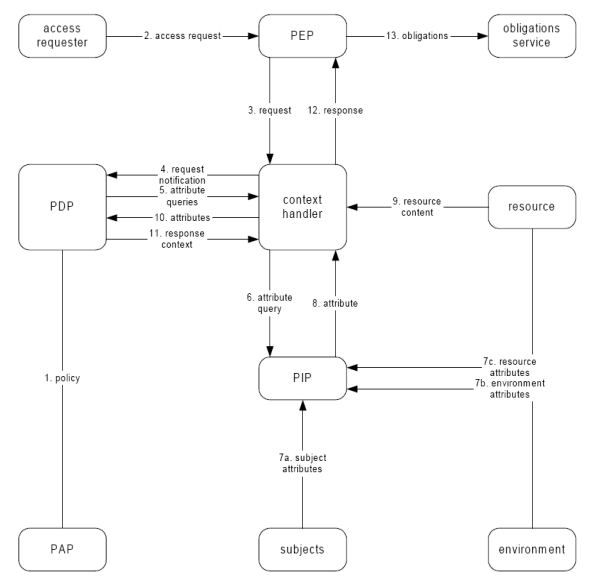
\includegraphics[scale=0.5]{07/XACML-Architecture.png}
            \caption{Architettura per il controllo degli accessi}
        \end{figure}
        
        Nella figura sopra possiamo vedere l'architettura per il controllo degli accessi con \texttt{XACML}. Questa architettura è composta da molte componenti che sono:
        \begin{description}
            \item[\texttt{PEP}]: \textit{Policy Enforcement Point} è l'entità che protegge la risorsa ed è il componente gli accesi facendo decisioni basate sulle richieste e facendo rispettare le decisioni.
            \item[\textit{Context Handler}]: è l'entità canonica che rappresenta di una decisione di accesso e autorizzazione. Viene designato alla conversione delle richieste da forma nativa a forma \texttt{XACML} e viceversa.
            \item[\texttt{PDP}]: \textit{Policy Decision Point} è l'entità che riceve e esamina le richieste, ricerca le \textit{policy} applicabili a quella richiesta, valuta le regole e invia la decisione di autorizzazione al \texttt{PEP}.
            \item[\texttt{PAP}]: \textit{Policy Administration Point} è l'entità che si occupa della gestione e conservazione delle \textit{policy} e delle regole.
            \item[\texttt{PIP}]: \textit{Policy Information Point} è l'entità che funge da sorgente degli attributi e dei dati necessari per valutare le \textit{policy}.
        \end{description}
\section{\texttt{OAUTH 2.0}}
    \texttt{OAUTH 2.0} è un protocollo di autorizzazione che permette di delegare solo certe autorizzazioni per l'accesso ad una risorsa. Ad esempio se si vuole fornire l'accesso ad una terza applicazione verso una risorsa di un utente, si può utilizzare \texttt{OAUTH 2.0} per delegare l'accesso a quella risorsa senza condividere le credenziali dell'utente.
    \paragraph{Flow Basico}
        \begin{enumerate}
            \item \textbf{Autenticazione}: l'utente si autentica presso il \textit{Resource Owner}. (non fa parte di \texttt{OAUTH 2.0})
            \item \textbf{Consenso Utente}: l'utente autorizza l'applicazione terza ad accedere per suo conto alla risorsa in questione.
            \item \textbf{Ricezione del Token}: il \textit{Resource Owner} genera un \texttt{OAuth Token} che contiene i permessi che l'utente ha concesso all'applicazione terza.
            \item \textbf{Accesso alla risorsa}: l'applicazione terza utilizza il \texttt{OAuth Token} per accedere alla risorsa.
        \end{enumerate}
    \paragraph{Flow di Autorizzazione}
        \begin{enumerate}
            \item Il \textit{client} ridirige il \textit{Resource Owner} all'\textit{endpoint} del \textit{Authorization Server}.
            \item Il \textit{Resource Owner} si autentica presso il \textit{Authorization Server}.
            \item Il \textit{Resource Owner} autorizza il \textit{client}
            \item A questo punto il \textit{Authorization Server} redirige il \textit{Resource Owner} al \textit{client} con un \texttt{authorization code}, questo non è il vero \texttt{token} per accedere alla risorsa ma è un \textit{token} che permette al \textit{client} di ottenere il \texttt{token} vero e proprio.
            \item Il \textit{client} invia il \texttt{authorization code} al \textit{Authorization Server} per ottenere il \texttt{token}, inoltre il \textit{client} deve autenticarsi presso il \textit{Authorization Server}.
            \item Il \textit{Authorization Server} invia una \texttt{OAuth access token} al \textit{client}.
            \item Il \textit{client} utilizza il \texttt{OAuth access token} per accedere alla risorsa.
        \end{enumerate}
    \subsection{Entità coinvolte}
        \subsubsection{\textit{Resourse Owner}}
            Questo è il proprietario della risorsa, generalmente è una persona che delega l'accesso a questa.
        \subsubsection{\textit{Protected Resource}}
            Queste risorse sono protette da parte del \textit{service provider} per conto del proprietario, le condivide solamente su richiesta di quest'ultimo.
        \subsubsection{\textit{Client}, App}
            Questa è l'applicazione che intende accedere alla risorsa, questo agisce come se fosse il proprietario su questa, ma solo dopo l'autorizzazione di quest'ultimo.
        \subsubsection{\textit{Authorization Server}}
            Questo \textit{server} è il responsabile per l'autenticazione dell'utente e per l'autenticazione delle risorse. È anche il responsabile per la gestione delle autorizzazioni ed genera un \textit{token} nel caso di autenticazione affermativa.
        \subsubsection{\textit{OAuth token}}
            Questo \textit{token} rappresenta le autorizzazioni delegate, come anticipato è generato dal'\textit{Authorization Server} ed è usato dal \textit{Client}
    \subsection{Note}
        Il protocollo è generalmente definito solo per \texttt{HTTP}, quindi per una comunicazione sicura viene usato \texttt{TLS}. \texttt{OAuth 2.0} non è un protocollo di autenticazione, ma dipende da questo in vari punti, questo non nega il fatto che i protocolli di autenticazione come \textit{OpenID Connect} si basino su \texttt{OAuth}.
        \subsubsection{Autenticazione con \texttt{OpenID Connect}}
            In quanto usare \texttt{OAuth 2.0} per il processo di autenticazione non è appropriato, in quanto l'utente deve essere presente solo al primo accesso, viene introdotto \texttt{OpenID Connect} 
\section{\texttt{JWT} - \textit{JSON Web Token}}
    \texttt{JWT} ovvero \textit{JSON Web Token} è uno standard aperto che definisce un modo compatto e autonomo per trasmettere informazioni tra due parti. Questo standard è usabile di fatto anche per \texttt{OAuth 2.0}, in quanto permette di trasmettere informazioni tra due parti in modo sicuro e firmato.
    \paragraph{Struttura}
        Un \texttt{JWT} è composto da tre parti separate da un punto:
        \begin{itemize}
            \item \textbf{Header}: contiene il tipo di token e l'algoritmo di firma.
            \item \textbf{Payload}: contiene le informazioni che si vogliono trasmettere come ad esempio l'identità dell'utente.
            \item \textbf{Signature}: contiene la firma del token, questa viene generata utilizzando l'header, il payload e una chiave segreta. Questa firma permette di verificare l'integrità del token, ma non permette di verificare la confidenzialità e l'autenticità.
        \end{itemize}
        La concatenazione di queste tre parti forma il \textit{token} \texttt{JWT}.
    \paragraph{Punti di forza}
        In quanto \texttt{JSON} è molto meno verboso di \texttt{XML} quando codificato è anche molto più leggero, il che lo rende ideale per essere trasportato in \texttt{HTTP} e \texttt{HTML}. Allo stesso modo \texttt{SAML} e \texttt{JWT} possono essere usati come coppia di chiave pubblica/privata nella forma di un certificato \texttt{X.509} per firmare e verificare i token.